\ifdefined\activerhandout 
\documentclass[12pt,aspectratio=1610,handout]{beamer}
\else
\documentclass[12pt,aspectratio=1610]{beamer}
\fi

%\usepackage[french]{babel} %=> erreur avec les tikz du moteur
\usepackage[T1]{fontenc}
\usepackage[utf8]{inputenc}
\usepackage{lmodern}
\usepackage{hyperref}
\usepackage{smartdiagram}
\usepackage{tikz}
\usepackage{animate}
\usepackage{tikzpeople}
\usepackage{appendixnumberbeamer}
\usepackage[labelformat=empty]{caption}
%\usepackage{pictochrono}
\usepackage{fontawesome5}
\usepackage{awesomebox}

\usetheme{Warsaw}
\setbeamertemplate{page number in head/foot}[totalframenumber]

\newcommand{\anglais}[1]{(\textit{\color{blue}#1})}
\newcommand{\legende}[2]{\caption[#1 (Source : \cite{#2})]{#1}}
\newcommand{\histoire}[1]{\begin{awesomeblock}{2pt}{\faBook}{black!75}#1\end{awesomeblock}}
\newcommand{\info}[1]{\begin{awesomeblock}{2pt}{\faInfoCircle}{black!75}#1\end{awesomeblock}}
\newcommand{\question}[1]{\begin{awesomeblock}{2pt}{\faQuestionCircle}{black!75}#1\end{awesomeblock}}
\newcommand{\alerte}[1]{\begin{awesomeblock}{2pt}{\faExclamationCircle}{black!75}#1\end{awesomeblock}}
\newcommand{\astuce}[1]{\begin{awesomeblock}{2pt}{\faLightbulb}{black!75}#1\end{awesomeblock}}
\newcommand{\exemple}[1]{\begin{awesomeblock}{2pt}{\faSearch}{black!75}#1\end{awesomeblock}}
\newcommand{\definitionAConnaitre}[1]{\begin{awesomeblock}{2pt}{\faCog}{black!75}#1\end{awesomeblock}}

\newcommand{\qmcBia}[7]{
%1 : titre slide
%2 : numéro de la bonne réponse
%3 : Inititulé de la question
%4, 5, 6, et 7 : propositions de réponse
\begin{frame}{#1}
\begin{awesomeblock}{2pt}{\faQuestion}{black!75}
#3
	\begin{enumerate}
	\ifnum#2=1
		\only<1>{\item #4}
		\only<2>{\item \textbf{#4}}
	\else
		\item #4
	\fi
	\ifnum#2=2
		\only<1>{\item #5}
		\only<2>{\item \textbf{#5}}
	\else
		\item #5
	\fi
	\ifnum#2=3
		\only<1>{\item #6}
		\only<2>{\item \textbf{#6}}
	\else
		\item #6
	\fi
	\ifnum#2=4
		\only<1>{\item #7}
		\only<2>{\item \textbf{#7}}
	\else
		\item #7
	\fi
	\end{enumerate}
	\pause
\end{awesomeblock}
\end{frame}
}

\subtitle{BIA - Brevet d'Initiation Aéronautique}
\author{Clément \textsc{Vermot-Desroches}}
\institute{Collège Aliénor d'Aquitaine\\Martignas-sur-Jalle}
\date{\today}

%\AtBeginSection[]
%{
%    \begin{frame}
%        %\frametitle{Table of Contents}
%        \tableofcontents[currentsection]
%    \end{frame}
%}

\AtBeginSubsection[]
{
    \begin{frame}
        %\frametitle{Table of Contents}
        \tableofcontents[currentsection,currentsubsection]
    \end{frame}
}

\title[Séance 4 - Commandes de vol]{Séance 4 \\ Commandes de vol}

\begin{document}
 \begin{frame}
 \titlepage
 \end{frame}
 
 \begin{frame}
 \tableofcontents
 \end{frame}
 
 \section{Les axes}
	\begin{frame}{Axes - Question}
	
	\question{Sur quels axes peut évoluer un aéronef ?}
	\pause
	\question{Comment le pilote peut-il intervenir sur ces axes ?}
	\pause
	\question{Qu'es-ce qui permet, sur l'aéronef, d'agir sur ces axes ?}
	\end{frame}	 

 	\begin{frame}{Les axes sur un aéronef}
		\begin{figure}[H]
  			\only<1| handout:0>{\includegraphics[scale=1]{imgPresentations/axes.pdf}}
  			\only<2>{\includegraphics[scale=1]{01-EtudeAeronefs/img/axes.pdf}}
  			\legende{Les axes sur un aéronef}{img:axes}	
  			\pause
		\end{figure}
	\end{frame}	
	
\section{Commandes de vol}
	\begin{frame}{Commandes de vol - axes du roulis}
	\begin{columns}
 	\begin{column}{0.5\textwidth}
	La commande sur l'axe du roulis (inclinaison gauche-droite) est obtenue par :
	\begin{itemize}
		\item une action latérale sur le manche
		\item provoquant un déplacement des ailerons
		\item montée de l'aileron du côté du virage, descente de l'aileron opposé.
	\end{itemize}
	\end{column}
	\begin{column}{0.5\textwidth}
		\begin{figure}[H]
  			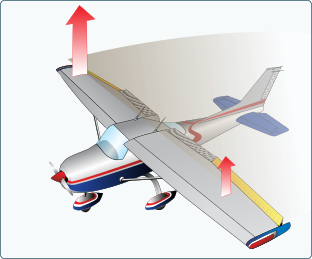
\includegraphics[width=1\textwidth]{01-EtudeAeronefs/img/virage.pdf}
  			\legende{Mise en virage à gauche}{img:virage}	
		\end{figure}	
	\end{column}
	\end{columns}
	\end{frame}
	
	\begin{frame}{Commandes de vol - axes du roulis - lacet inverse}
	\begin{columns}
	\begin{column}{0.5\textwidth}
		\begin{figure}[H]
  			\includegraphics[width=1\textwidth]{01-EtudeAeronefs/img/lacetInverse.pdf}
  			\legende{Lacet inverse (à droite pour un virage à gauche)}{img:lacetInverse}	
		\end{figure}	
	\end{column}
 	\begin{column}{0.5\textwidth}
	La trainée supplémentaire créée par l'augmentation de la portance provoque un lacet dans sens inverse au virage
	\end{column}
	\end{columns}
	\end{frame}
	
	\begin{frame}{Commandes de vol - axes du tangage}
	\begin{columns}
 	\begin{column}{0.5\textwidth}
	La commande sur l'axe du tangage (avant-arrière) est obtenue par :
	\begin{itemize}
		\item une action longitudinale sur le manche,
		\item provoquant un déplacement de la gouverne de profondeur,
		\item la gouverne monte quand on tire sur la manche, et descend quand on pousse,
		\item la gouverne de profondeur est \textbf{déportante}.
	\end{itemize}
	\end{column}
	\begin{column}{0.5\textwidth}
		\begin{figure}[H]
  			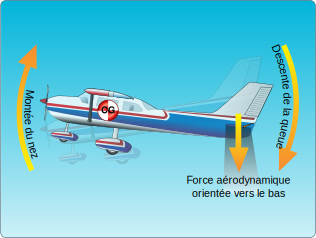
\includegraphics[width=1\textwidth]{01-EtudeAeronefs/img/gouverneProfondeur.pdf}
  			\legende{Commande de profondeur}{img:gouverneProfondeur}	
		\end{figure}	
	\end{column}
	\end{columns}
	\end{frame}
	
	\begin{frame}{Commandes de vol - axes du lacet}
	\begin{columns}
	\begin{column}{0.5\textwidth}
		\begin{figure}[H]
  			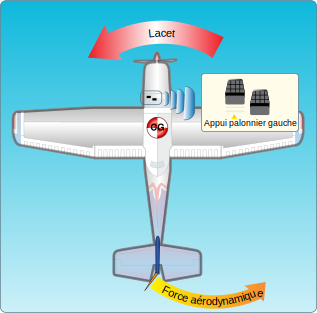
\includegraphics[width=1\textwidth]{01-EtudeAeronefs/img/gouverneDeDirection.pdf}
  			\legende{Commande de profondeur}{img:gouverneDeDirection}	
		\end{figure}	
	\end{column}
	\begin{column}{0.5\textwidth}
	La commande sur l'axe du lacet (latéral) est obtenue par :
	\begin{itemize}
		\item une action sur le palonnier (pédale)
		\item provoquant un déplacement de la gouverne de direction
		\item la gouverne se déplace du côté de l'appui.
	\end{itemize}
	\end{column}
	\end{columns}
	\end{frame}
	
	\begin{frame}{Actionnement des commandes de vol}
	Sur des avions légers et peu rapide, le lien entre le manche et les surface de contrôle de est réalisé grâce à des jeux de câbles, poulies et renvois.
	
		\begin{figure}[H]
  			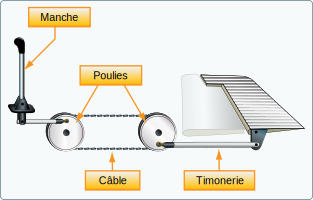
\includegraphics[width=0.6\textwidth]{01-EtudeAeronefs/img/cdvMecaniques.pdf}
  			\legende{Commande de vol mécaniques}{img:cdvMecaniques}	
		\end{figure}	
	
	\end{frame}
	
	\begin{frame}{Actionnement des commandes de vol}
	Sur des avions plus lourds ou plus rapide, la taille des surfaces de contrôle devient importante. Les efforts aux commandes de vol deviennent importants. On assiste donc les commandes de vol via des systèmes hydrauliques.
	
	
		\begin{figure}[H]
  			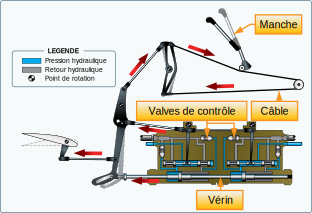
\includegraphics[width=0.55\textwidth]{01-EtudeAeronefs/img/cdvHydrauliques.pdf}
  			\legende{Commande de vol hydrauliques}{img:cdvHydrauliques}	
		\end{figure}	
	
	
	\end{frame}
	
	\begin{frame}{Commandes de vol électriques}
		\begin{itemize}
			\item Suppression du lien physique entre le manche et les gouvernes
			\item Les actions des pilotes sont acheminées vers des ordinateurs
			\item Protègent "l'enveloppe de vol" : 
			\begin{itemize}
				\item empêche le décrochage
				\item empêche d'incliner trop fortement/rapidement l'avion
			\end{itemize}
			\item Rendre pilotable des avions volontairement conçus instables (chasseurs)
		\end{itemize}
		
		\histoire{Premier avion commercial avec commandes de vol électriques : Concorde (1976)
		
		 Puis tous les avions Airbus à partir de l'A320 (1987)}
	\end{frame}
	
	\begin{frame}{Commandes de vol électriques}
		\begin{figure}[H]
  			\includegraphics[width=0.7\textwidth]{01-EtudeAeronefs/img/cdve.png}
  			\legende{Commande de vol électriques}{img:cdve}	
		\end{figure}	
	\end{frame}

%TODO satabilité (centrage, compensateur ?)
\begin{frame}{Stabilité - centre de gravite}
	\begin{figure}[H]
  		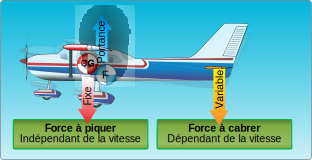
\includegraphics[width=0.8\textwidth]{04-Aerodynamique/img/centrage.pdf}
  		\legende{Position centre de gravité - foyer}{img:centrage}	
	\end{figure}	
\end{frame}

 
\appendix 
\section{QCM}
\qmcBia{Étude des aéronefs}
{1}{Quels sont les éléments présents dans une commande de vol mécanique simple d'un avion d'aéroclub ?}
{Câbles et poulies}
{Tuyaux hydrauliques et servo-commande}
{Moteurs électriques et câbles}
{Bielles et pistons} 
{}

\qmcBia{Étude des aéronefs}
{3}{Pour effectuer une rotation autour de l'axe de roulis, le pilote doit :}
{modifier la profondeur à l'aide du compensateur}
{déplacer le manche en avant ou en arrière}
{déplacer le manche à gauche ou à droite}
{actionner le palonnier} 
{}

\qmcBia{Étude des aéronefs}
{3}{Lorsque le pilote incline le manche à droite :}
{les ailerons se lèvent}
{les ailerons de baissent}
{l'aileron droit se lève et l'aileron gauche se baisse}
{l'aileron gauche se lève et l'aileron droit se baisse} 
{On veut augmenter la portance sur l'aile gauche, et la diminuer à droite.}

\qmcBia{Étude des aéronefs}
{1}{En avion, l'action qui permet une rotation autour de l'axe de tangage est :	}
{un déplacement en avant ou en arrière du manche}
{un déplacement latéral du manche}
{une poussée à gauche ou à droite sur les palonniers}
{un déplacement latéral du manche et simultanément une poussée des palonniers} 
{}
 
\ifdefined\activerbibliobeamer
\begin{frame}[allowframebreaks]
\frametitle{Bibliographie}
\printbibliography
%\nocite{*}
\end{frame}
\fi 
 
\end{document}
